\documentclass{acm_proc_article-sp}
\makeatletter
\let\@copyrightspace\relax
\makeatother

\newcommand{\thetitle}{Predicting Network Flow Behavior From Five Packets}

%!TEX root = paper.tex

\usepackage[labelfont=bf,small]{caption}
\usepackage[font=small,labelfont=bf,position=top,nearskip=0em]{subfig}
\usepackage{cite,amsmath,amssymb,rotating,multirow,bigstrut,url,wrapfig,relsize,paralist,array,mathtools,units}
\usepackage[hyperfigures,bookmarks,bookmarksopen,bookmarksnumbered,colorlinks,linkcolor=black,citecolor=black,filecolor=blue,menucolor=black,pagecolor=blue,frenchlinks=true,pdftitle={\thetitle}]{hyperref}

%!TEX root = paper.tex

%% LABELING COMMANDS
\renewcommand{\sec}[1]{\label{sec:#1}}
\newcommand{\eqn}[1]{\label{eqn:#1}}
\newcommand{\fig}[1]{\label{fig:#1}}
\newcommand{\tab}[1]{\label{tab:#1}}
\newcommand{\thm}[1]{\label{thm:#1}}
\newcommand{\defn}[1]{\label{def:#1}}

%% REFERENCING COMMANDS
\newcommand{\Appendix}[1]{\hyperref[sec:#1]{Appendix~\ref*{sec:#1}}}
\newcommand{\Section}[1]{\hyperref[sec:#1]{Section~\ref*{sec:#1}}}
\newcommand{\Equation}[1]{\hyperref[eqn:#1]{Equation~\ref*{eqn:#1}}}
\newcommand{\Figure}[1]{\hyperref[fig:#1]{Figure~\ref*{fig:#1}}}
\newcommand{\Table}[1]{\hyperref[tab:#1]{Table~\ref*{tab:#1}}}
\newcommand{\Theorem}[1]{\hyperref[thm:#1]{Theorem~\ref*{thm:#1}}}
\newcommand{\Definition}[1]{\hyperref[def:#1]{Definition~\ref*{def:#1}}}

%% MATHEMATICAL NOTATIONS

% common algebraic domains
\newcommand{\N}{\mathbb{N}}
\newcommand{\Z}{\mathbb{Z}}
\newcommand{\Q}{\mathbb{Q}}
\newcommand{\R}{\mathbb{R}}

% standard operators & functors
\renewcommand{\Pr}{\mathrm{Pr}}
\newcommand{\Image}{\text{Im}}
\newcommand{\Kernel}{\text{Ker}}

% common constructs
\newcommand{\abs}[1]{{\left|#1\right|}}
\newcommand{\absx}[1]{{|#1|}}
\newcommand{\card}[1]{{\left|#1\right|}}
\newcommand{\cardx}[1]{{|#1|}}
\newcommand{\norm}[1]{{\lVert#1\rVert}}
\newcommand{\normx}[1]{{\Vert#1\Vert}}
\newcommand{\set}[1]{{\left\{#1\right\}}}
\newcommand{\setx}[1]{{\{#1\}}}
\newcommand{\parens}[1]{{\left(#1\right)}}
\newcommand{\parensx}[1]{{(#1)}}
\newcommand{\bracket}[1]{{\left[#1\right]}}
\newcommand{\bracketx}[1]{{[#1]}}
\newcommand{\seq}[1]{{\left<#1\right>}}
\newcommand{\seqx}[1]{{\lvert#1\rvert}}
\newcommand{\tuple}[1]{{\left<#1\right>}}
\newcommand{\tuplex}[1]{{\lvert#1\rvert}}
\newcommand{\floor}[1]{{\left\lfloor#1\right\rfloor}}
\newcommand{\floorx}[1]{{\lfloor#1\rfloor}}
\newcommand{\ceil}[1]{{\left\lceil#1\right\rceil}}
\newcommand{\ceilx}[1]{{\lceil#1\rceil}}
\newcommand{\round}[1]{{\left[#1\right]}}
\newcommand{\roundx}[1]{{[#1]}}
\newcommand{\fracx}[2]{{#1/#2}}
\newcommand{\fracp}[2]{{\left(\frac{#1}{#2}\right)}}
\newcommand{\fracpx}[2]{{(#1/#2)}}
\newcommand{\smallfrac}[2]{{\textstyle{\frac{#1}{#2}}}}

% standard notations
\newcommand{\trans}[1]{{#1}^T}
\newcommand{\inner}[2]{{#1}\trans{#2}}
\newcommand{\cross}{\times}
\newcommand{\tensor}{\otimes}
\newcommand{\directsum}{\oplus}
\newcommand{\iso}{\cong}
\newcommand{\union}{\cup}
\newcommand{\inter}{\cap}
\newcommand{\disunion}{\sqcup}
\newcommand{\Union}{\bigcup}
\newcommand{\Inter}{\bigcap}
\newcommand{\Disunion}{\bigsqcup}
\newcommand{\conj}{\wedge}
\newcommand{\disj}{\vee}
\newcommand{\Conj}{\bigwedge}
\newcommand{\Disj}{\bigvee}
\newcommand{\defeq}{=}
\renewcommand{\emptyset}{\varnothing}
\renewcommand{\setminus}{\,\raisebox{1pt}{$\smallsetminus$}\,}
\newcommand{\eldiv}{\,./\,}
\newcommand{\diag}{\text{diag}}
\newcommand{\rs}{\text{rs}}
\newcommand{\argmin}{\text{arg min}}

%% FORMATTING BEHAVIORS
\newcommand{\caps}[1]{{\small{#1}}}
\newcommand{\latin}[1]{\textit{#1}}
\newcommand{\defterm}[1]{\textit{#1}}
\newcommand{\newfootnote}[2]{\newcommand{#1}{\footnote{#2} }}
\renewcommand{\bullet}{\raisebox{2pt}{$\centerdot$}}
\renewcommand{\arraystretch}{1.3}

%% MISCELLANEOUS

\renewcommand{\vec}[1]{\mathbf{#1}}


\title{\vspace{-1em}\thetitle}
\author{
{Stefan~Karpinski, John~R.~Gilbert, Elizabeth~M.~Belding} \vspace{0.75em}\\
Department of Computer Science \\
University of California, Santa Barbara \vspace{0.75em}\\
{\{sgk,gilbert,ebelding\}@cs.ucsb.edu}
}

\newcommand{\figurename}{Figure}
\newcommand{\tablename}{Table}

\begin{document}
\maketitle

\begin{abstract}
We observe that when network traffic behaviors are represented in vector spaces as relative frequency histograms of behavioral features, they exhibit low-rank linear structure.
We hypothesize that this structure is due to the distribution of flow behaviors following a  finite mixture model.
Aside from being of theoretical interest, this hypothesis has practical consequences:
it allows us to make predictions about the probabilities of future flow behaviors from a handful of a flow's initial packets.
From observing five initial packets, we are able to predict the distribution of future packet sizes and inter-packet intervals with between 70\% and 90\% accuracy across a variety of network traces.
We can predict which flow will have more packets in pairwise comparisons with between 65\% and 85\% accuracy.
These practical applications serve dual functions.
They provide highly useful tools for network management, routing decisions, and quality of service schemes.
However, they also provide evidence that the hypothesized model gives a correct explanation for the observed linear structure in real network traffic.
\end{abstract}

\section*{Extended Abstract}

\newfootnote{\flownote}{We use the common definition of a \textit{flow} as a sequence of packets sharing the same  ``5-tuple'': IP protocol type, source and destination nodes, and TCP/UDP port numbers.}
\newfootnote{\directsumnote}{Direct sum is the vector space analogue of cross product.}

This work begins with a particular way of representing flow behaviors as vectors.
The representation is quite simple.
For each feature of a flow, we represent that aspect of the flow's behavior as a \emph{feature-frequency vector}:
a vector having a dimension for each possible value of the feature and whose coordinates are the relative frequency of values.
For example, the vector for the distribution of packet sizes of a flow with four 40-byte and two 145-bytes packets is
\begin{align}
  \text{size} = \frac{1}{4+2}\parens{4\vec{e}_{40} + 2\vec{e}_{145}}.
\end{align}
% The dimension of this representation is 1500 because that is typically the maximum transfer unit (\caps{MTU}) of local networks.
Different aspects of flow behavior can be represented in this way, and these representations can be combined by taking the direct sum of their representation vectors:
\begin{align}\eqn{flow}
  \text{flow} =
  \text{size} \directsum
  \text{ival} \directsum
  \text{type} \directsum
  \text{port} \directsum
  \text{pkts}.
\end{align}
The features here are packet size and inter-packet interval distributions, \caps{IP} protocol type, source and destination port numbers, and packet count.
The behavior of a feature across a collection of flows can be expressed as a matrix where each row represents a flow:
\begin{align}\eqn{Size}
  \text{Size} = \bracket{ ~\text{size}_1~ ; ~\cdots~ ; ~\text{size}_m~ }.
\end{align}
The overall behavior of the collection of flows then becomes a concatenation of these feature matrices:
\begin{align}\eqn{X}
  X = \bracket{ ~
    \text{Size} ~
    \text{Ival} ~
    \text{Type} ~
    \text{Port} ~
    \text{Pkts} ~
  }.
\end{align}
% It is this matrix, representing the total behavior of a collection of flows, to which we apply our analysis.
When traffic traces are represented like this, a very curious thing happens:
the resulting matrices exhibit a great deal of linear structure.
Specifically, flow behaviors tend to lie near the union of a small set of low-rank subspaces.
\Figure{svd}~shows this structure visually.
These scatter plots show the first two most significant dimensions of the behavior matrix after reduction via singular value decomposition (\caps{SVD}) and projection onto the unit-sum hyperplane.

\begin{figure}[t]
\vspace{-0.9em}
\begin{center}
\subfloat[\scriptsize{DART.}]{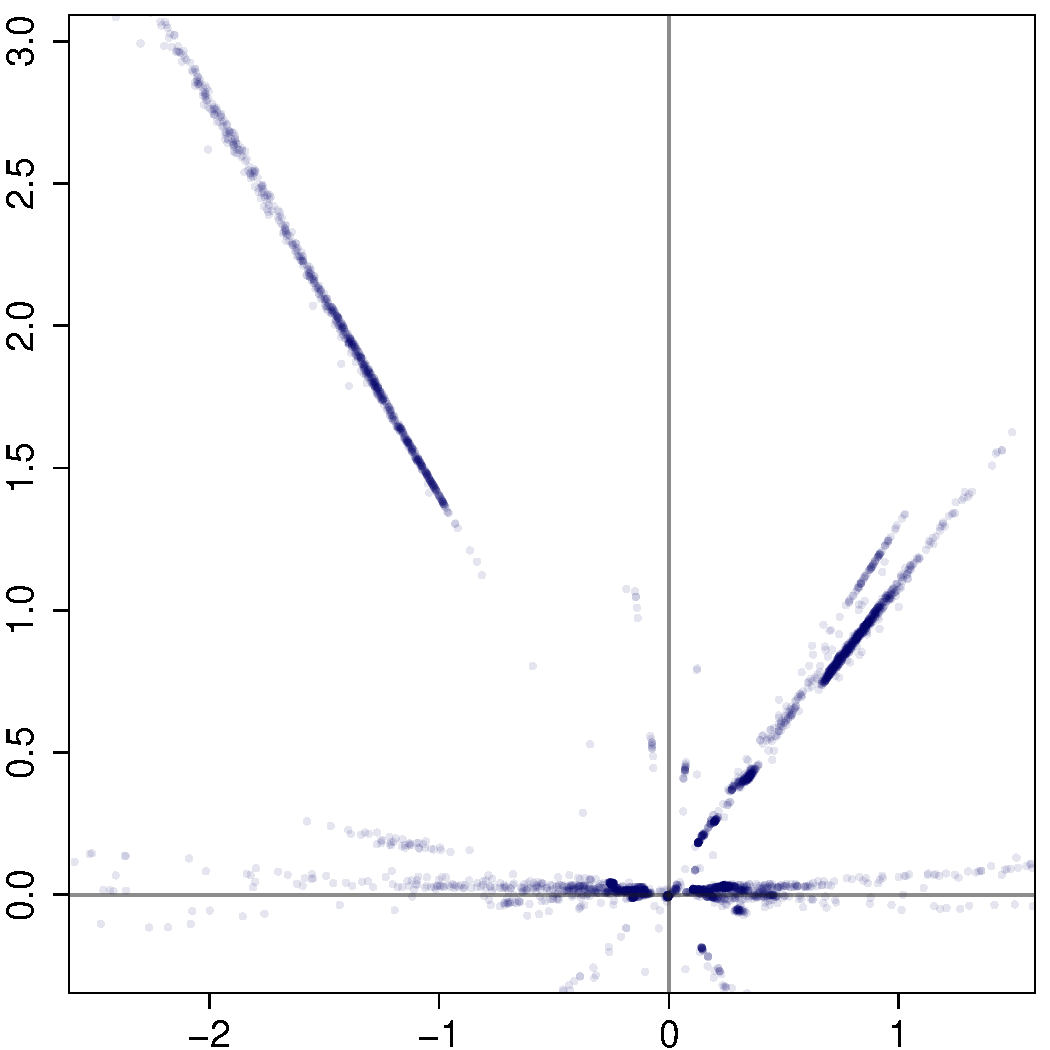
\includegraphics[width=1.059in]{svd/dart}}
% \subfloat[\scriptsize{IETF 60}]{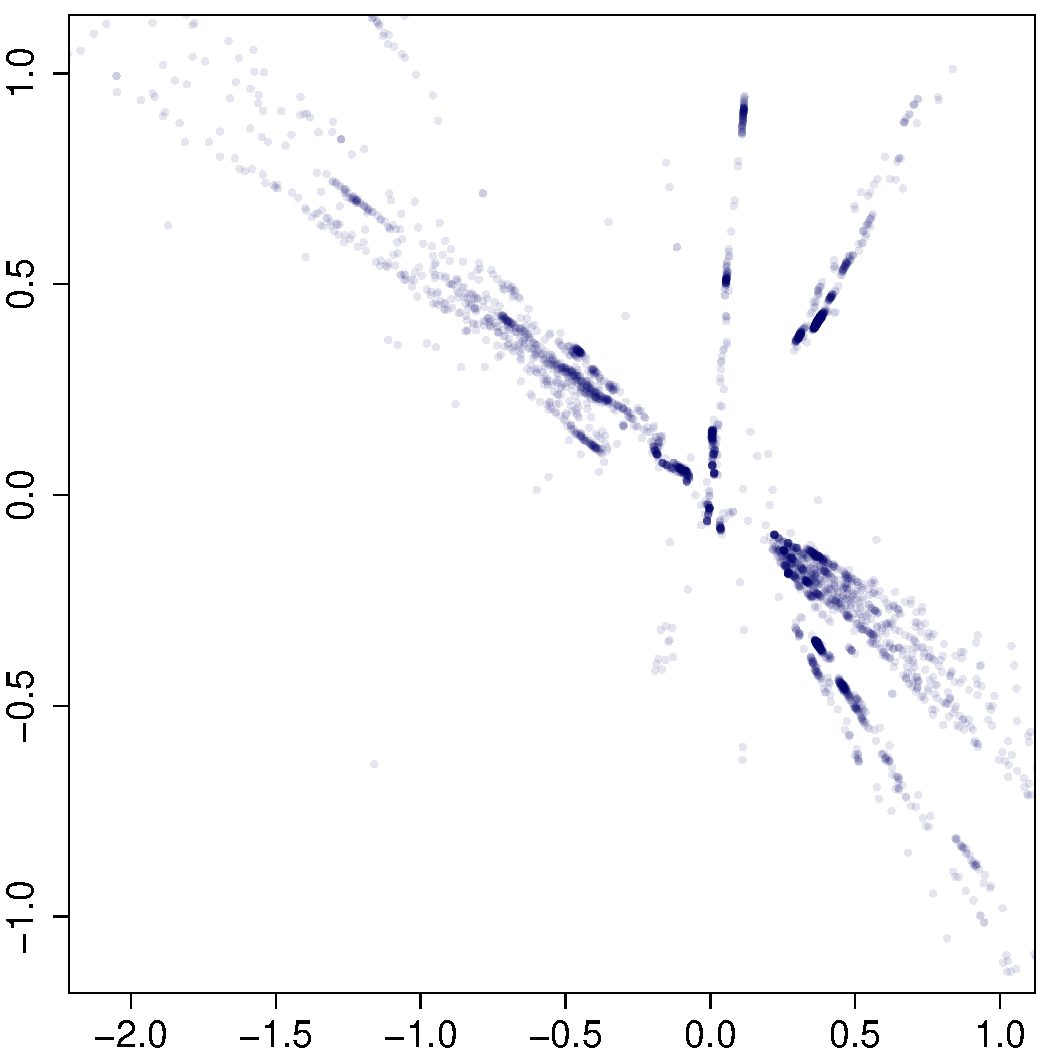
\includegraphics[width=1.059in]{svd/ie60}}
% \subfloat[\scriptsize{SIGCOMM 2004}]{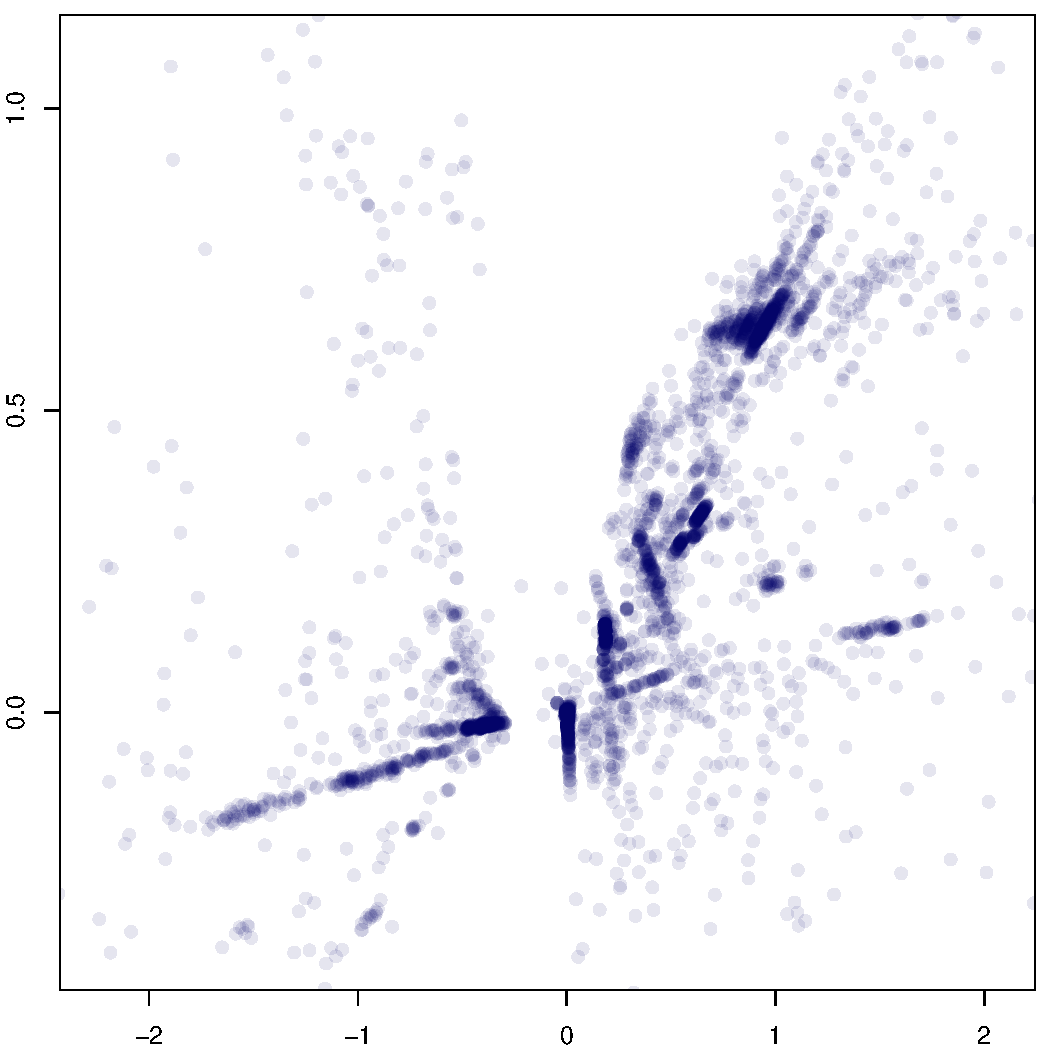
\includegraphics[width=1.059in]{svd/sc04}}
\subfloat[\scriptsize{IETF 67}]{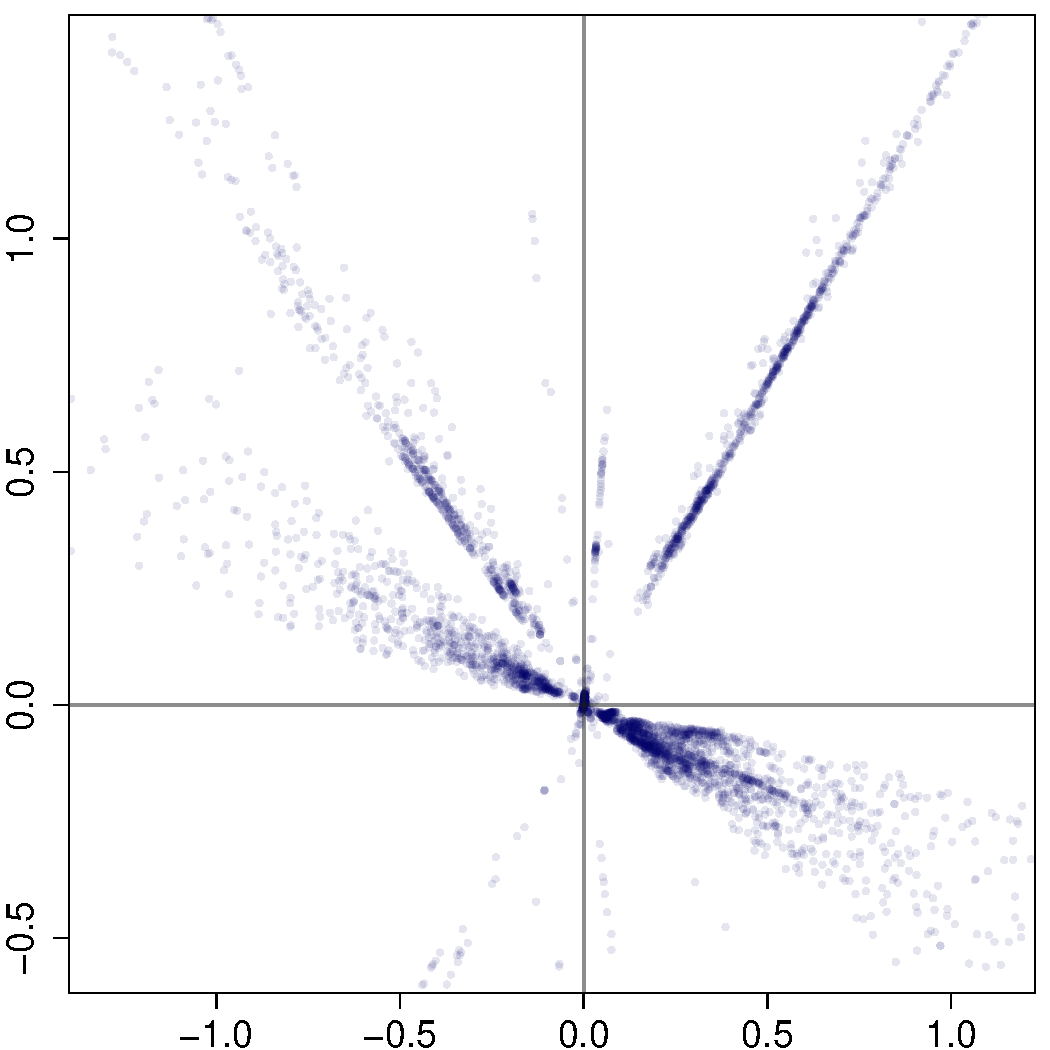
\includegraphics[width=1.059in]{svd/ie67}}
% \subfloat[\scriptsize{SIGCOMM 2001}]{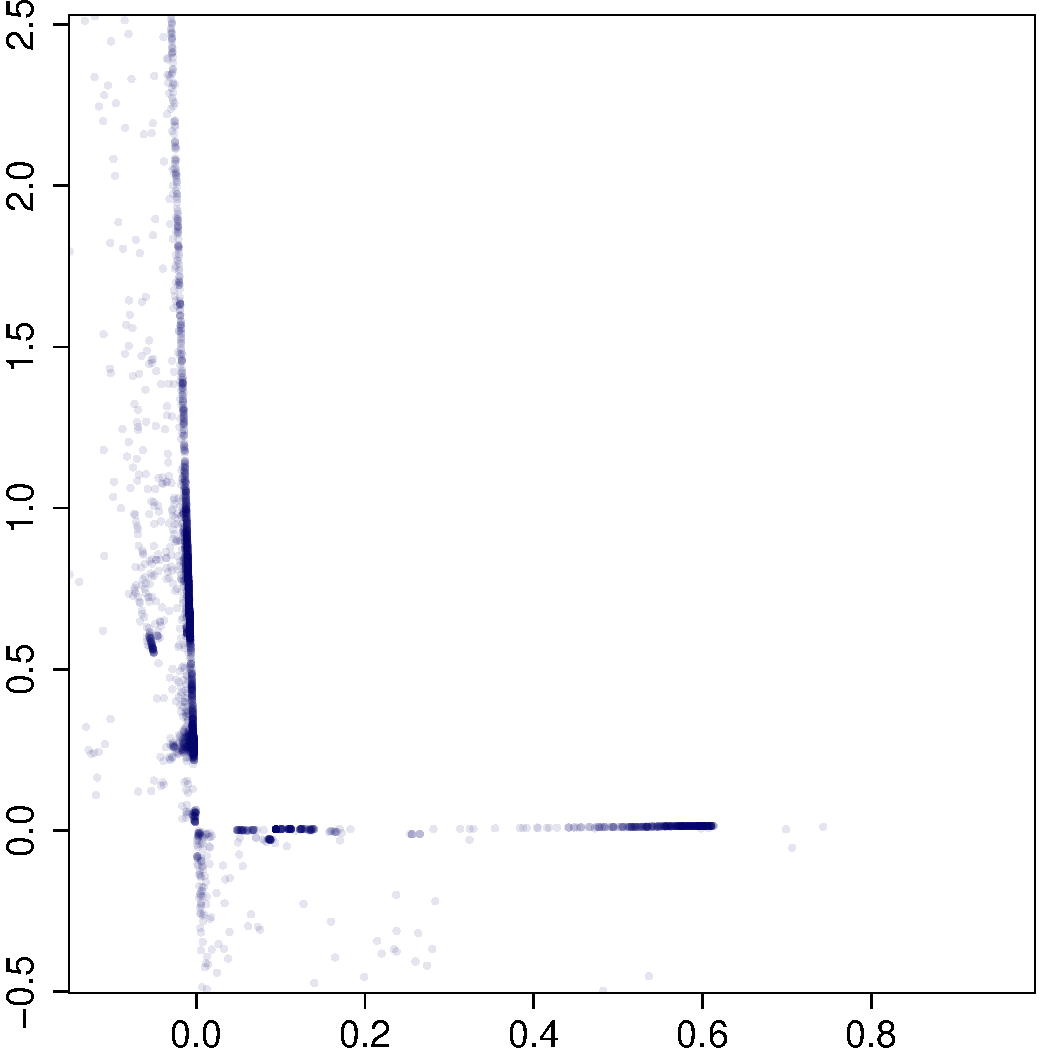
\includegraphics[width=1.059in]{svd/sc01}}
\subfloat[\scriptsize{UCSD}]{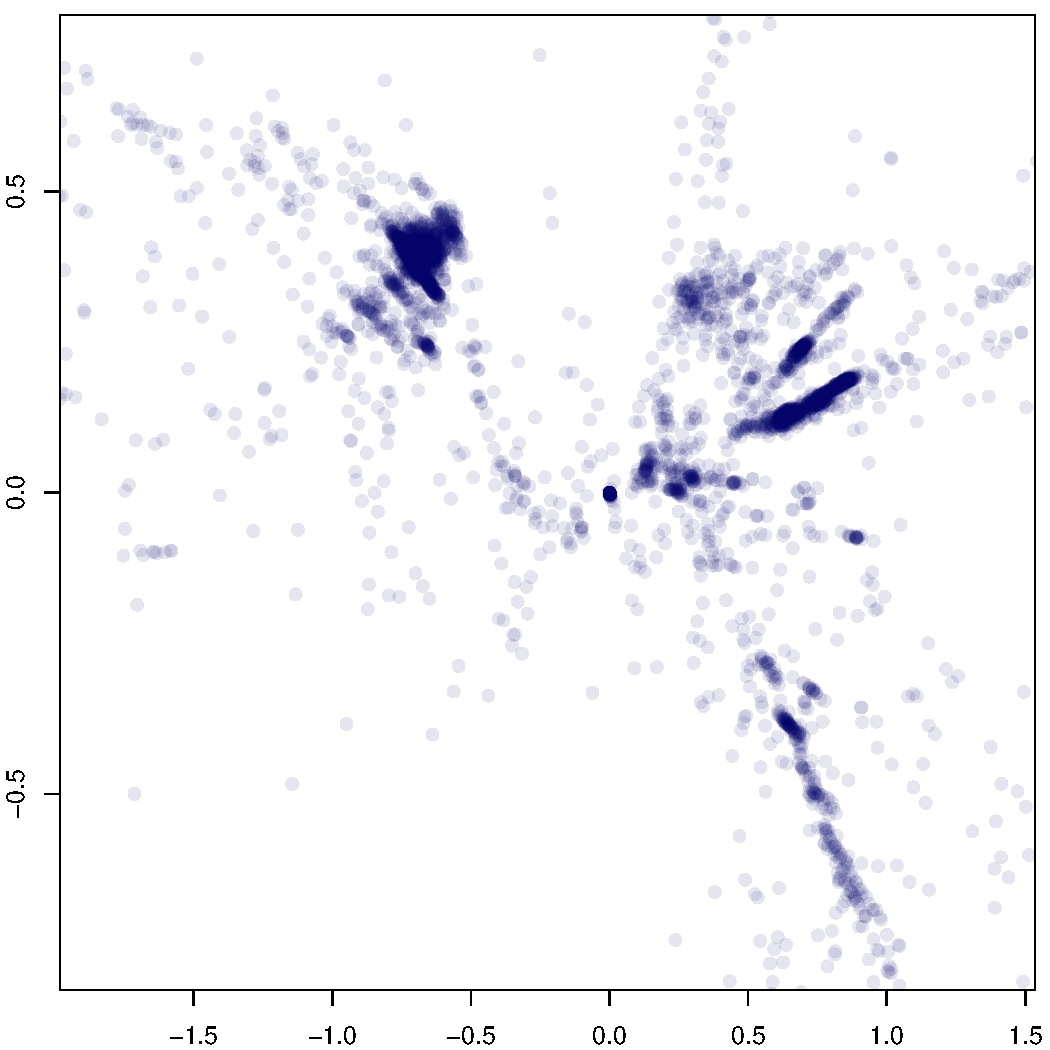
\includegraphics[width=1.059in]{svd/ucsd}}
\caption{Scatter plots of the two most significant SVD dimensions of the feature-frequency representations of traffic samples from the six network traffic traces analyzed in our experiments.} 
\fig{svd}
\end{center}
\vspace{-2em}
\end{figure}

% We hypothesize that the reason for the linear structure is that the distribution of each flows behavior is a finite mixture of a small set of ``basic behaviors.''
% Moreover, the mixing of basic behaviors is itself structured.
% The linear structure of network traffic allows us to perform a drastic model reduction on trace traffic patterns while preserving the essential characteristics of the original trace.
% Furthermore, when observable characteristics of flows are separated from features to be predicted, this model reduction is similar to a classical linear regression:
% it allows us to use least squares optimization on observed features to predict individual flow behavior.
% We use this technique to predict the following characteristics of flows from a few initial packets.

To explain this linear structure, we hypothesize that the behavior distribution for most flows is a mixture of a small set of ``basic behaviors.''
Moreover, only even smaller subsets of these basic behaviors are typically combined with each other.
Under these assumptions, we can express the distribution of each flow's behaviors as a finite mixture model~\cite{McLachlan00}:
\begin{align}\eqn{mixture-model}
  q_i(x) = \sum_{j=1}^r w_{ij} p_j(x).
\end{align}
Here $q_i$ and $p_j$ are probability density functions, and $w_{ij}$ are nonnegative weights, summing to unity for each $i$.
\Equation{mixture-model} is expressed succinctly as matrix multiplication.
Writing $Q_{ik} = q_i(k)$, $W_{ij} = w_{ij}$, and $P_{jk} = p_j(k)$, we have:
\begin{align}\eqn{mixture-model-matrix}
  Q = WP.
\end{align}
The number of basic behaviors, $r$, is the maximum possible rank of the feature distribution matrix, $Q$.
Moreover, we can partition the rows of $P$ into classes such that $w_{ij_1}$ and $w_{ij_2}$ are both non-zero only if $j_1$ and $j_2$ are in the same class.
Thus, each row of $Q$ is associated with exactly one class, and all the points associated with a class lie in the subspace spanned by its associated rows in $P$.

This model explains the structures in \Figure{svd}.
Points along the same low-rank structure are in the same class.
A structure is ``generated'' by a small set of vertices:
points belonging to a structure are near the hull of its vertices.
This is only one possible hypothesis that fits the data.
Like any hypothesis, it must be tested.
Our prediction technique, aside from providing a practical application, serves as a hypothesis test:
we try to recover the matrices $W$ and $P$ from our noisy and imperfect observations of $Q$ and use the recovered model to predict real flow behaviors.
If the recovered model can make accurate predictions, this provides evidence that our model and hypothesis approximate reality.

% This prediction technique is clearly of immediate practical use:
% applications range from network management to routing to quality of service.
% Looking deeper than these applications, however, the mere fact that this prediction technique works at all provides evidence that the underlying hypothesized model of flow behavior is valid.
% Our future works will provide evidence and applications by applying this model to the problems of traffic classification and realistic workload generation.

% Our experimental procedure has three parts:
% training, prediction and evaluation.
% For training, we take samples of network traces and attempt to recover the parameters of the hypothesized model.
% We use the recovered model to predict behaviors of a separate set of flows from the same trace, using only knowledge of five initial packets from each flow.
% Finally, we must evaluate the quality of these predictions by comparing them against the actual behavior of those flows.

From training data we recover estimates, $W^*$ and $P^*$, of the factors in \Equation{mixture-model-matrix}.
To detect the low-rank linear structures, we use Ma~\emph{et~al.}'s algorithm for segmenting multivariate data into subspaces using lossy data coding and compression~\cite{Ma07}.
Then we determine the hull points of each linear structure using nonnegative matrix factorization (\caps{NMF})~\cite{Lee01,Kim08:anls}:
if $Q_c$ is a sub-matrix of rows in the same structure class, we want to find nonnegative matrices, $W_c$ and $P_c$, such that $Q_c \approx W_c P_c$.
Our reconstructed $P^*$ is a vertical concatenation of these $P_c$ matrices, while $W^*$ is a row-permutation of the direct sum of $W_c$ matrices.
We use Kim and Park's alternating non-negative least squares algorithm~\cite{Kim08:anls} for rapid initial convergence, but refine the result using Lee and Seung's Euclidean algorithm~\cite{Lee01}.
Good prediction performance requires special initialization of the \caps{NMF} algorithms, using new techniques that we lack room to detail here.

To predict flow behavior, we separate flow features into those observed and those to be predicted:
\begin{align}
  X_\text{o} &= \bracket{ ~
    \text{Size}_\text{init} ~
    \text{Ival}_\text{init} ~
    \text{Type} ~
    \text{Port} ~
  }, \\
  X_\text{p} &= \bracket{ ~
    \text{Size}_\text{rest} ~
    \text{Ival}_\text{rest} ~
    \text{Pkts} ~
  }.
\end{align}
$\text{Size}_\text{init}$ is the packet size matrix for the first five packets, while $\text{Size}_\text{rest}$ is the matrix for the remainder of the packets, and similarly for inter-packet intervals.
From an observation matrix, $X_\text{o}$, and the recovered model parameters, $P^*$, we can make predictions about $X_\text{p}$.
Let $P^* = \bracketx{P^*_\text{o}~P^*_\text{p}}$ be the recovered model parameter matrix  with separated observable and predictable features.
From an observation matrix for test data, $X_\text{o}$, we estimate the matrix of weights by minimizing the squared Frobenius error:
\begin{align}
  W^* = \text{argmin}_W {\norm{X_\text{o} - W P^*_\text{o}}^2_\text{frob}}
\end{align}
with the constraint that $W$ be nonnegative.
We can estimate the underlying feature distributions for the flows:
\begin{align}
  Q^* = W^*P^*.
\end{align}
The ``predictable'' portion, $Q^*_\text{p}$, contains predictions of packet size distribution, inter-packet interval distribution and distribution of packet counts for each flow.
To evaluate the quality of these predictions, we compare the distributions in $Q^*_\text{p}$ to the matrix, $X_\text{p}$, of actual test flow behaviors.

\begin{table}
\vspace{0.05em}
\begin{center}
\scriptsize
\begin{tabular}{|c|c|c|c|}

\hline
\textbf{Trace} &
\textbf{Year} &
\textbf{Type} &
\textbf{Network} \\
\hline

{\scriptsize{DARTMOUTH}} &
2003 &
campus &
Dartmouth College \\
\hline

{\scriptsize{IETF 60}} &
2004 &
conference &
IETF hotel \\
\hline

{\scriptsize{IETF 67}} &
2006 &
conference &
IETF hotel \\
\hline

{\scriptsize{SIGCOMM 2001}} &
2001 &
conference &
SIGCOMM hotel \\
\hline

{\scriptsize{SIGCOMM 2004}} &
2004 &
conference &
SIGCOMM hotel \\
\hline

{\scriptsize{UCSD}} &
2007 &
campus &
UCSD engineering \\
\hline

\end{tabular}
\caption{Traffic traces used for analysis and experiments.}
\tab{traces}
\end{center}
\vspace{-2em}
\end{table}

\begin{figure}[t]
\begin{center}
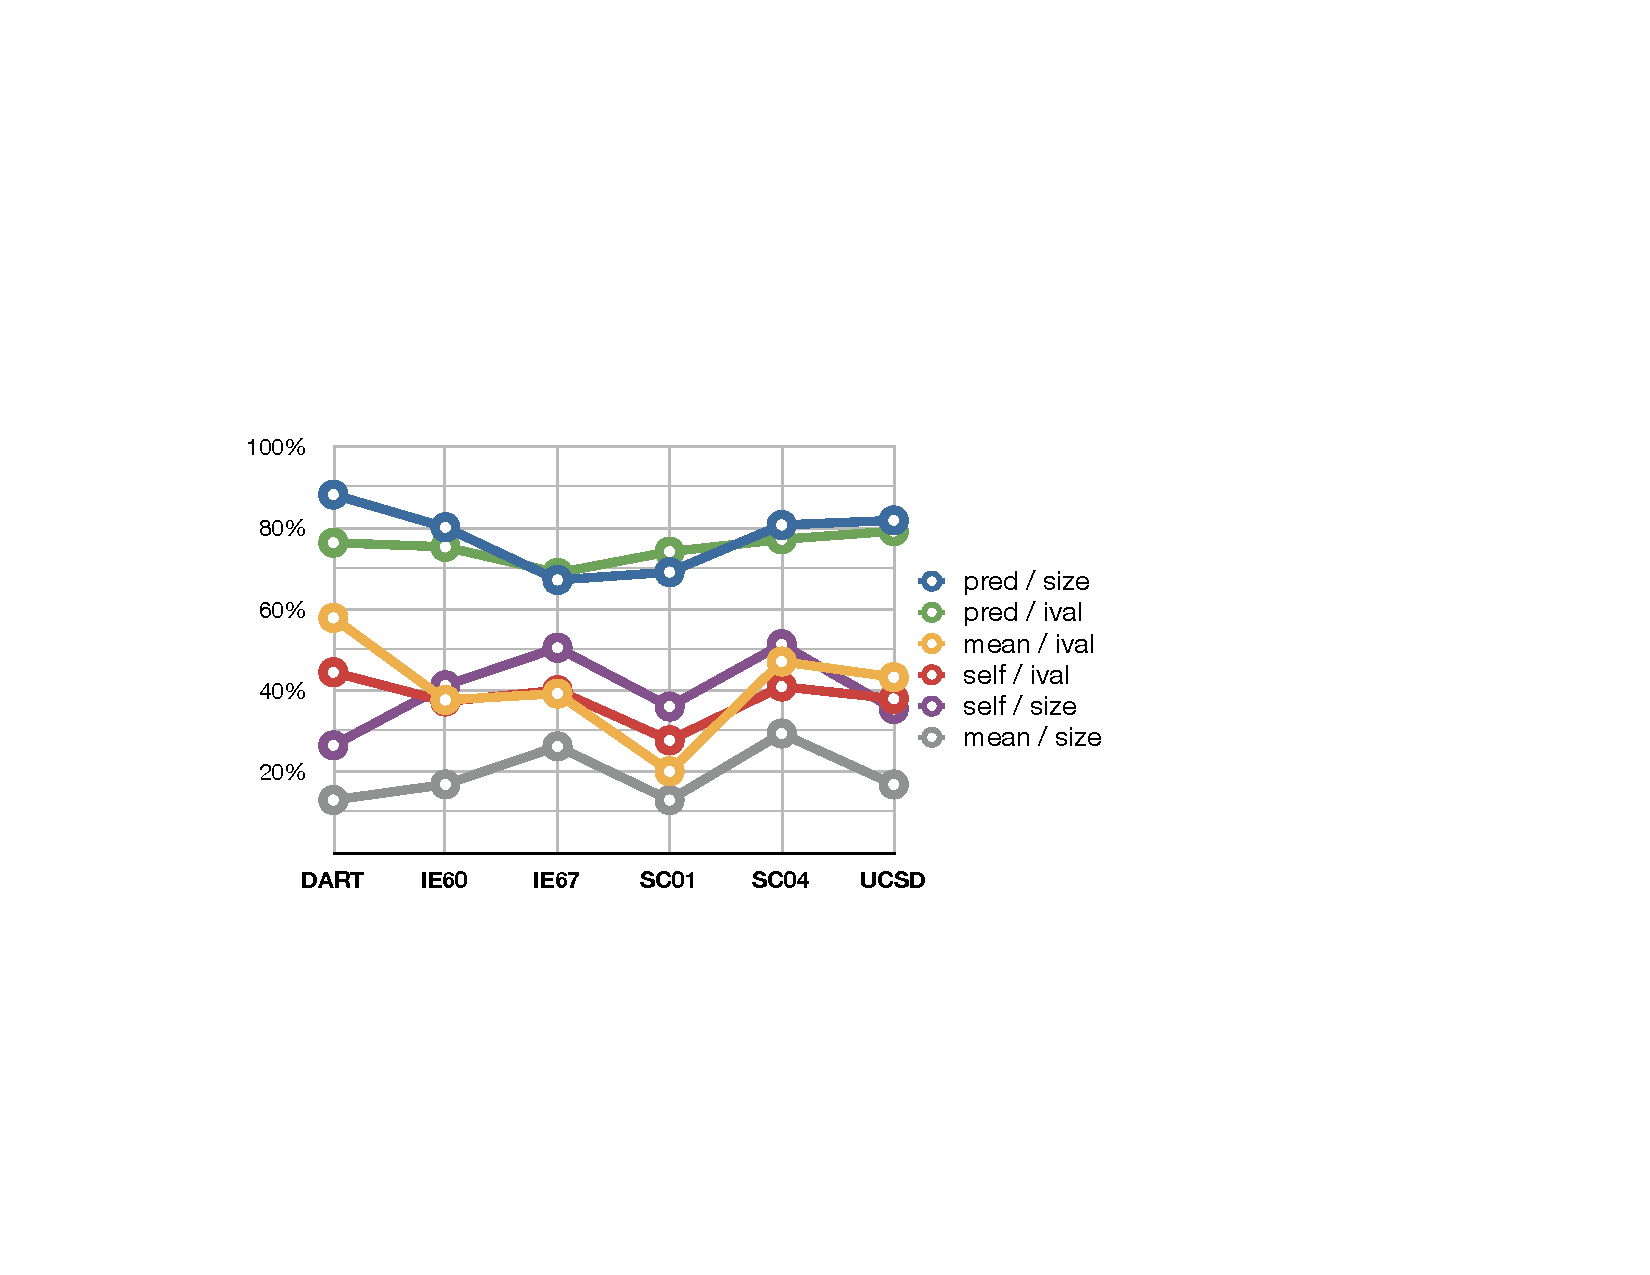
\includegraphics[width=3.3in]{pred_stats}
\caption{Accuracy rates of various methods of predicting flow behavior from five initial packets across six data sets.}
\fig{accuracy}
\end{center}
\vspace{-2em}
\end{figure}

For our experiments, we use randomly sampled traffic from six network traces.
The traces are freely available from the \caps{CRAWDAD} trace repository~\cite{Yeo06}.
Details of the traces are shown in \Table{traces}.
% These data sets represent a broad cross-section of traffic patterns over time and a reasonable variety of network types.
% Unfortunately, we could not find any freely available residential or corporate network traces that were usable for our analysis.
We randomly sampled 5000 flows from each trace for training and another 5000 flows for testing.
% Since the initial five packets are used for prediction, we consider only flows with at least five packets.
The results are shown in \Figure{accuracy}.
The left panel shows the accuracy rates of predicting packet size and inter-packet interval distributions.
Accuracy is computed by comparing the distribution of Kolmogorov-Smirnov (K-S) test p-values to an empirical ideal distribution of K-S p-values, taking the maximum deviation from the ideal as the error rate.
Since no previous work attempts to either model individual flow behavior or predict flow behavior from initial observations, we compare our prediction technique to two simple and obvious approaches:
predicting the already observed behavior of each flow, and
predicting the average behavior of the training trace.
The right-top panel shows the accuracy rate for predicting which flow will have more packets between random pairs of flows.
Choosing randomly gives 50\% accuracy, which we exceed significantly on all traces.

Our method does not yield perfect predictions, but the non-deterministic nature of flow behavior implies that it is impossible to achieve perfect prediction.
Moreover, we do not know what the inherent upper limit on prediction quality is:
no prior work provides detailed statistical models of individual flow behaviors, nor does any earlier research attempt to predict individual flow behavior from a few initial packets.
The fact that this technique can accurately predict flow behavior from so few initial packet observations is evidence that our hypothesized mixture model for flow behavior has merit.
With improvements in the algorithms used to recover the model parameters, we are confident that even better prediction accuracy can be achieved.
Furthermore, the same model can be applied to traffic classification from flow behavior, and to generation of realistic synthetic network traffic from collections of trace data.
These applications, however useful, are merely pleasant side effects of the real breakthrough of this work:
a detailed statistical model for individual flow behaviors across whole networks.

\scriptsize
\bibliographystyle{unsrt}
\bibliography{references}

\end{document}
